\chapter{Results: Comparing CDA and FBA}
\label{ch:results}
% AUTO-GENERATED by analysis/make_tables.py -- do not hand-edit.
% Re-run `python analysis/run_all.py` to regenerate after the
% underlying results/sol/*.csv change.

\newcommand{\DescBookImbalanceCdaMean}{0.0199}
\newcommand{\DescBookImbalanceCdaMedian}{0.0350}
\newcommand{\DescBookImbalanceCdaN}{2,655,219}
\newcommand{\DescBookImbalanceCdaStd}{0.6189}
\newcommand{\DescBoundaryConcentrationFbaMean}{0.1014}
\newcommand{\DescBoundaryConcentrationFbaMedian}{0.0658}
\newcommand{\DescBoundaryConcentrationFbaN}{2,654,665}
\newcommand{\DescBoundaryConcentrationFbaStd}{0.1188}
\newcommand{\DescResidualShareFbaMean}{0.9618}
\newcommand{\DescResidualShareFbaMedian}{1.0000}
\newcommand{\DescResidualShareFbaN}{2,677,996}
\newcommand{\DescResidualShareFbaStd}{0.1389}
\newcommand{\DescTotalBookDepthCdaMean}{720,058.53}
\newcommand{\DescTotalBookDepthCdaMedian}{579,162.25}
\newcommand{\DescTotalBookDepthCdaN}{2,655,219}
\newcommand{\DescTotalBookDepthCdaStd}{354,817.51}
\newcommand{\DispersionFbaExactZeroPct}{96.58}
\newcommand{\DispersionFbaNonzeroPct}{3.42}
\newcommand{\FbaEmptyBatchShare}{76.62}
\newcommand{\LatencyCdaPNinetyNine}{2.97}
\newcommand{\LatencyFbaPNinetyNine}{3,721.00}
\newcommand{\PriceDiffMeanBps}{-0.00}
\newcommand{\PriceDiffMedianBps}{0.00}
\newcommand{\PriceDiffN}{545,573}
\newcommand{\PriceDiffStdBps}{0.85}
\newcommand{\PricepathsDay}{2025-12-18}
\newcommand{\ResAmihudCda}{0.09}
\newcommand{\ResAmihudDiff}{0.02}
\newcommand{\ResAmihudFba}{0.11}
\newcommand{\ResAmihudHacSe}{0.00}
\newcommand{\ResAmihudNPaired}{545,572}
\newcommand{\ResAmihudP}{$<$0.001}
\newcommand{\ResClearingLatencyCda}{1.25}
\newcommand{\ResClearingLatencyDiff}{1,916.75}
\newcommand{\ResClearingLatencyFba}{1,918.00}
\newcommand{\ResClearingLatencyHacSe}{4.03}
\newcommand{\ResClearingLatencyNPaired}{2,655,207}
\newcommand{\ResClearingLatencyP}{$<$0.001}
\newcommand{\ResDepthAtBestCda}{133.40}
\newcommand{\ResDepthAtBestDiff}{280.90}
\newcommand{\ResDepthAtBestFba}{414.30}
\newcommand{\ResDepthAtBestHacSe}{1.83}
\newcommand{\ResDepthAtBestNPaired}{2,655,207}
\newcommand{\ResDepthAtBestP}{$<$0.001}
\newcommand{\ResDepthWithinFiftyBpsCda}{158,346.57}
\newcommand{\ResDepthWithinFiftyBpsDiff}{-2,114.44}
\newcommand{\ResDepthWithinFiftyBpsFba}{156,232.12}
\newcommand{\ResDepthWithinFiftyBpsHacSe}{50.18}
\newcommand{\ResDepthWithinFiftyBpsNPaired}{2,655,207}
\newcommand{\ResDepthWithinFiftyBpsP}{$<$0.001}
\newcommand{\ResDepthWithinHundredBpsCda}{268,437.06}
\newcommand{\ResDepthWithinHundredBpsDiff}{-7,500.16}
\newcommand{\ResDepthWithinHundredBpsFba}{260,936.90}
\newcommand{\ResDepthWithinHundredBpsHacSe}{143.50}
\newcommand{\ResDepthWithinHundredBpsNPaired}{2,655,207}
\newcommand{\ResDepthWithinHundredBpsP}{$<$0.001}
\newcommand{\ResDepthWithinTenBpsCda}{32,681.93}
\newcommand{\ResDepthWithinTenBpsDiff}{-1,166.17}
\newcommand{\ResDepthWithinTenBpsFba}{31,515.77}
\newcommand{\ResDepthWithinTenBpsHacSe}{8.03}
\newcommand{\ResDepthWithinTenBpsNPaired}{2,655,207}
\newcommand{\ResDepthWithinTenBpsP}{$<$0.001}
\newcommand{\ResDispersionCda}{0.17}
\newcommand{\ResDispersionDiff}{-0.15}
\newcommand{\ResDispersionFba}{0.03}
\newcommand{\ResDispersionHacSe}{0.00}
\newcommand{\ResDispersionNPaired}{545,573}
\newcommand{\ResDispersionP}{$<$0.001}
\newcommand{\ResEffectiveSpreadCda}{1.00}
\newcommand{\ResEffectiveSpreadDiff}{1.68}
\newcommand{\ResEffectiveSpreadFba}{2.68}
\newcommand{\ResEffectiveSpreadHacSe}{0.01}
\newcommand{\ResEffectiveSpreadNPaired}{545,562}
\newcommand{\ResEffectiveSpreadP}{$<$0.001}
\newcommand{\ResExecNotionalCda}{7,541.95}
\newcommand{\ResExecNotionalDiff}{40.54}
\newcommand{\ResExecNotionalFba}{7,582.49}
\newcommand{\ResExecNotionalHacSe}{29.73}
\newcommand{\ResExecNotionalNPaired}{2,678,400}
\newcommand{\ResExecNotionalP}{0.173}
\newcommand{\ResExecVolumeCda}{58.08}
\newcommand{\ResExecVolumeDiff}{0.29}
\newcommand{\ResExecVolumeFba}{58.37}
\newcommand{\ResExecVolumeHacSe}{0.23}
\newcommand{\ResExecVolumeNPaired}{2,678,400}
\newcommand{\ResExecVolumeP}{0.215}
\newcommand{\ResFillRateCda}{0.0029}
\newcommand{\ResFillRateDiff}{0.0000}
\newcommand{\ResFillRateFba}{0.0030}
\newcommand{\ResFillRateHacSe}{0.0000}
\newcommand{\ResFillRateNPaired}{2,654,250}
\newcommand{\ResFillRateP}{$<$0.001}
\newcommand{\ResKyleLambdaCda}{0.09}
\newcommand{\ResKyleLambdaDiff}{-0.09}
\newcommand{\ResKyleLambdaFba}{0.00}
\newcommand{\ResKyleLambdaHacSe}{0.00}
\newcommand{\ResKyleLambdaNPaired}{633,632}
\newcommand{\ResKyleLambdaP}{$<$0.001}
\newcommand{\ResOrderToTradeRatioCda}{208.3221}
\newcommand{\ResOrderToTradeRatioDiff}{-17.1751}
\newcommand{\ResOrderToTradeRatioFba}{191.1471}
\newcommand{\ResOrderToTradeRatioHacSe}{0.2141}
\newcommand{\ResOrderToTradeRatioNPaired}{545,573}
\newcommand{\ResOrderToTradeRatioP}{$<$0.001}
\newcommand{\ResPriceImpactFiveSCda}{1.52}
\newcommand{\ResPriceImpactFiveSDiff}{-3.35}
\newcommand{\ResPriceImpactFiveSFba}{-1.83}
\newcommand{\ResPriceImpactFiveSHacSe}{0.03}
\newcommand{\ResPriceImpactFiveSNPaired}{545,562}
\newcommand{\ResPriceImpactFiveSP}{$<$0.001}
\newcommand{\ResPriceImpactOneSCda}{1.33}
\newcommand{\ResPriceImpactOneSDiff}{-0.61}
\newcommand{\ResPriceImpactOneSFba}{0.71}
\newcommand{\ResPriceImpactOneSHacSe}{0.01}
\newcommand{\ResPriceImpactOneSNPaired}{545,562}
\newcommand{\ResPriceImpactOneSP}{$<$0.001}
\newcommand{\ResPriceImpactThirtySCda}{1.65}
\newcommand{\ResPriceImpactThirtySDiff}{-10.40}
\newcommand{\ResPriceImpactThirtySFba}{-8.75}
\newcommand{\ResPriceImpactThirtySHacSe}{0.08}
\newcommand{\ResPriceImpactThirtySNPaired}{545,561}
\newcommand{\ResPriceImpactThirtySP}{$<$0.001}
\newcommand{\ResQuotedSpreadCda}{0.84}
\newcommand{\ResQuotedSpreadDiff}{0.03}
\newcommand{\ResQuotedSpreadFba}{0.87}
\newcommand{\ResQuotedSpreadHacSe}{0.00}
\newcommand{\ResQuotedSpreadNPaired}{2,655,207}
\newcommand{\ResQuotedSpreadP}{$<$0.001}
\newcommand{\ResRealizedSpreadFiveSCda}{-0.51}
\newcommand{\ResRealizedSpreadFiveSDiff}{5.03}
\newcommand{\ResRealizedSpreadFiveSFba}{4.51}
\newcommand{\ResRealizedSpreadFiveSHacSe}{0.03}
\newcommand{\ResRealizedSpreadFiveSNPaired}{545,562}
\newcommand{\ResRealizedSpreadFiveSP}{$<$0.001}
\newcommand{\ResRealizedSpreadOneSCda}{-0.32}
\newcommand{\ResRealizedSpreadOneSDiff}{2.29}
\newcommand{\ResRealizedSpreadOneSFba}{1.97}
\newcommand{\ResRealizedSpreadOneSHacSe}{0.01}
\newcommand{\ResRealizedSpreadOneSNPaired}{545,562}
\newcommand{\ResRealizedSpreadOneSP}{$<$0.001}
\newcommand{\ResRealizedSpreadThirtySCda}{-0.65}
\newcommand{\ResRealizedSpreadThirtySDiff}{12.08}
\newcommand{\ResRealizedSpreadThirtySFba}{11.43}
\newcommand{\ResRealizedSpreadThirtySHacSe}{0.09}
\newcommand{\ResRealizedSpreadThirtySNPaired}{545,561}
\newcommand{\ResRealizedSpreadThirtySP}{$<$0.001}
\newcommand{\ResRealizedVolCda}{0.00}
\newcommand{\ResRealizedVolDiff}{0.00}
\newcommand{\ResRealizedVolFba}{0.00}
\newcommand{\ResRealizedVolHacSe}{n/a}
\newcommand{\ResRealizedVolNPaired}{1}
\newcommand{\ResRealizedVolP}{n/a}
\newcommand{\ResSizeInflationCda}{44.5535}
\newcommand{\ResSizeInflationDiff}{-6.5890}
\newcommand{\ResSizeInflationFba}{37.9645}
\newcommand{\ResSizeInflationHacSe}{0.3160}
\newcommand{\ResSizeInflationNPaired}{925,551}
\newcommand{\ResSizeInflationP}{$<$0.001}
\newcommand{\ResThroughputCda}{960,048.63}
\newcommand{\ResThroughputDiff}{-704,908.83}
\newcommand{\ResThroughputFba}{255,139.80}
\newcommand{\ResThroughputHacSe}{1,187.60}
\newcommand{\ResThroughputNPaired}{2,655,207}
\newcommand{\ResThroughputP}{$<$0.001}
\newcommand{\ResTimeToExecCda}{19.28}
\newcommand{\ResTimeToExecDiff}{3.52}
\newcommand{\ResTimeToExecFba}{22.80}
\newcommand{\ResTimeToExecHacSe}{0.07}
\newcommand{\ResTimeToExecNPaired}{925,551}
\newcommand{\ResTimeToExecP}{$<$0.001}
\newcommand{\ResTradeCountCda}{1.30}
\newcommand{\ResTradeCountDiff}{0.02}
\newcommand{\ResTradeCountFba}{1.32}
\newcommand{\ResTradeCountHacSe}{0.00}
\newcommand{\ResTradeCountNPaired}{2,678,400}
\newcommand{\ResTradeCountP}{$<$0.001}
\newcommand{\ResTraderSurplusCda}{37.02}
\newcommand{\ResTraderSurplusDiff}{0.48}
\newcommand{\ResTraderSurplusFba}{37.51}
\newcommand{\ResTraderSurplusHacSe}{0.07}
\newcommand{\ResTraderSurplusNPaired}{2,678,400}
\newcommand{\ResTraderSurplusP}{$<$0.001}
\newcommand{\ResVwapCda}{129.84}
\newcommand{\ResVwapDiff}{0.00}
\newcommand{\ResVwapFba}{129.84}
\newcommand{\ResVwapHacSe}{0.00}
\newcommand{\ResVwapNPaired}{545,573}
\newcommand{\ResVwapP}{0.429}
\newcommand{\SampleCancellations}{281,778,306}
\newcommand{\SampleCdaNotional}{20,200,362,171.01}
\newcommand{\SampleCdaTrades}{3,481,516}
\newcommand{\SampleDistinctParticipants}{37,027}
\newcommand{\SampleFbaNotional}{20,308,937,215.80}
\newcommand{\SampleFbaTrades}{3,530,770}
\newcommand{\SampleFilesTotal}{744}
\newcommand{\SampleMeanInterArrival}{4.159}
\newcommand{\SampleMedianInterArrival}{0.000}
\newcommand{\SampleNewOrders}{283,797,135}
\newcommand{\SampleOtherEvents}{57,615,417}
\newcommand{\SamplePNinetyNineInterArrival}{126.6}
\newcommand{\SampleSkipped}{16,985,954}
\newcommand{\SampleSkippedPct}{2.58}
\newcommand{\SampleTotalMessages}{640,176,812}
\newcommand{\SampleZeroGapPct}{96.0}
\newcommand{\ValCargoTestsPassed}{80}
\newcommand{\ValCargoTestsTotal}{80}
\newcommand{\ValChecklistPassed}{37}
\newcommand{\ValChecklistTotal}{37}
\newcommand{\ValInvariantViolations}{0}
\newcommand{\ValRunComplete}{true}


\begin{quote}
\small
\textbf{Scope of this chapter.} Every number and figure below comes from
one executed run: SOL/USD, the full month of 1--31~December 2025,
$\tau = 1$\,second, the single fixed engine configuration
\Cref{app:config} describes (\Cref{sec:experiments}). There is no
interval sweep, no rationing-rule comparison, and no second instrument
or session in this data --- \Cref{sec:res_sweep,sec:res_rationing} say
so explicitly where the original design called for them. Every
paired-difference statistic is computed only over the subset of
one-second intervals in which the metric was computable on \emph{both}
engines (a minority of the 2,678,400 intervals in the month, for most
metrics --- each table reports how many), using Newey--West standard
errors robust to autocorrelation (\Cref{sec:experiments}).
\end{quote}

\section{Sample and Descriptive Statistics}
\label{sec:sample}

\Cref{tab:sample} describes the replayed sample: one instrument, one
continuous month, the composition of the event stream that both engines
consume unchanged. Because the input is identical for both arms, this
table characterises what was fed to the comparison, and any asymmetry in
\Cref{sec:res21,sec:res22,sec:res23} cannot originate here. There is a
single column, not the liquid-pair/less-liquid-pair/high-volatility-session
breakdown an earlier draft of this table assumed: \Cref{sec:experiments}
explains why only one instrument and one session exist in this design.

\begin{table}[htbp]
\centering
\caption[Sample description]{Description of the replayed sample. Message
counts refer to the raw event stream, identical for both engines; trade
counts and notional are each engine's own simulated output.}
\label{tab:sample}
\small
\begin{tabularx}{\textwidth}{@{}L c@{}}
\toprule
\textbf{Characteristic} & \textbf{Value}\\
\midrule
Instrument & SOL/USD\\
Session & 1--31 Dec 2025 (\FbaEmptyBatchShare\% of 1s FBA batches empty)\\
Input files & \SampleFilesTotal\\
Total records seen & \SampleTotalMessages\\
\quad of which new live orders & \SampleNewOrders\\
\quad of which cancellations & \SampleCancellations\\
\quad of which other (rejections, fills, non-triggered conditionals) & \SampleOtherEvents\\
\quad skipped (zero size after rounding) & \SampleSkipped\ (\SampleSkippedPct\%)\\
Distinct participants (user ids) & \SampleDistinctParticipants\\
Median inter-arrival time, raw record stream & \SampleMedianInterArrival\,ms\\
Mean inter-arrival time & \SampleMeanInterArrival\,ms\\
99th pct.\ inter-arrival time & \SamplePNinetyNineInterArrival\,ms\\
CDA trades (simulated) & \SampleCdaTrades\\
FBA trades (simulated) & \SampleFbaTrades\\
CDA executed notional (simulated) & \$\SampleCdaNotional\\
FBA executed notional (simulated) & \$\SampleFbaNotional\\
\bottomrule
\end{tabularx}
\end{table}

There is no separate row for order modifications: the replayed data has
no distinct modify event, and neither engine implements one
(\Cref{sec:environment}) --- a change to a resting order surfaces as
some combination of the categories above, not as its own count.

The inter-arrival figures deserve a comment, because the median by
itself (\SampleMedianInterArrival\,ms, i.e.\ exactly zero at the
precision reported) understates what is happening: \SampleZeroGapPct\%
of consecutive records in the raw stream share the identical nanosecond
timestamp, consistent with the node logging several order-status events
--- e.g.\ both counterparties' fills from one match, or a cancel and its
replacement --- as one atomic write. The distribution is bimodal rather
than degenerate: the mean (\SampleMeanInterArrival\,ms) and the 99th
percentile (\SamplePNinetyNineInterArrival\,ms) show a substantial tail of
genuinely spaced-out arrivals between these bursts. Either figure is
still one to two orders of magnitude shorter than $\tau = 1$\,second, so
a typical batch accumulates many records rather than behaving as a
delayed CDA passing through at most one event at a time --- consistent
with the FBA's \FbaEmptyBatchShare\% empty-batch share reported above.

\section{Validation Results}
\label{sec:validationresults}

\Cref{tab:validation} reports the validation layers \Cref{sec:validation}
actually applies, and marks the two further checks that section
describes as not built rather than omitting them silently. These are
prerequisites, not findings: the comparison in the following sections is
only as interpretable as the harness that produced it.

\begin{table}[htbp]
\centering
\caption[Validation results]{Validation of the replay harness and both
engines, for the exact build used to produce this chapter's data.}
\label{tab:validation}
\small
\begin{tabularx}{\textwidth}{@{}L c@{}}
\toprule
\textbf{Validation check} & \textbf{Result}\\
\midrule
Process aborts (structural invariant violations) during this run & \ValInvariantViolations\\
Inline test suite passed (\texttt{cargo test}) & \ValCargoTestsPassed/\ValCargoTestsTotal\\
Hand-computed checklist passed (\texttt{test engine all}) & \ValChecklistPassed/\ValChecklistTotal\\
Run completed to \texttt{complete = true} & \ValRunComplete\\
Run-to-run determinism (byte-identical logs, single uninterrupted run) & yes, by construction; not independently re-verified for this run\\
CDA trade-for-trade agreement with venue output & not built --- \Cref{sec:validation}\\
FBA--CDA convergence in cleared volume as $\tau \to 0$ & not built --- requires the interval sweep, \Cref{sec:experiments}\\
\bottomrule
\end{tabularx}
\end{table}

The first four rows are direct evidence about this specific run and the
binary that produced it (\Cref{sec:validation}); the fifth restates that
determinism is a property of an uninterrupted run given fixed input, not
something re-checked bit-for-bit after the fact for a multi-day,
checkpointed run. The last two rows are not weaker results but absent
ones, and \Cref{sec:res21,sec:res22,sec:res23} should be read with that
in mind: nothing below confirms the CDA against the venue's own trades,
and nothing below demonstrates the FBA converging to the CDA as $\tau$
shrinks.

\section{RQ2.1: Liquidity and Transaction Costs}
\label{sec:res21}

\Cref{tab:res21} reports the liquidity and cost metrics of
\Cref{tab:metrics1} for both engines, with the paired difference
(FBA$-$CDA) and its Newey--West standard error and $p$-value, computed
only over intervals where both engines had a qualifying observation
(the $n$ column; \Cref{sec:experiments}, \Cref{app:formulas}).
Book imbalance and total book depth have no FBA analogue and are
reported as CDA-only descriptive statistics beneath the paired rows,
not as a difference.

\begin{table}[htbp]
\centering
\caption[RQ2.1 results]{Liquidity and transaction costs under both
mechanisms. Paired differences per interval (FBA$-$CDA); Newey--West
standard errors robust to autocorrelation in parentheses; $n$ is the
number of one-second intervals (of 2{,}678{,}400 in the month) in which
the metric was computable on both engines.}
\label{tab:res21}
\small
\begin{tabularx}{\textwidth}{@{}L c c c c c@{}}
\toprule
\textbf{Metric} & \textbf{CDA} & \textbf{FBA} & \textbf{Diff.} &
\textbf{$p$} & \textbf{$n$}\\
\midrule
Quoted spread (bps) & \ResQuotedSpreadCda & \ResQuotedSpreadFba & \ResQuotedSpreadDiff & \ResQuotedSpreadP & \ResQuotedSpreadNPaired\\
Depth at best & \ResDepthAtBestCda & \ResDepthAtBestFba & \ResDepthAtBestDiff & \ResDepthAtBestP & \ResDepthAtBestNPaired\\
Depth within 10 bps & \ResDepthWithinTenBpsCda & \ResDepthWithinTenBpsFba & \ResDepthWithinTenBpsDiff & \ResDepthWithinTenBpsP & \ResDepthWithinTenBpsNPaired\\
Depth within 50 bps & \ResDepthWithinFiftyBpsCda & \ResDepthWithinFiftyBpsFba & \ResDepthWithinFiftyBpsDiff & \ResDepthWithinFiftyBpsP & \ResDepthWithinFiftyBpsNPaired\\
Depth within 100 bps & \ResDepthWithinHundredBpsCda & \ResDepthWithinHundredBpsFba & \ResDepthWithinHundredBpsDiff & \ResDepthWithinHundredBpsP & \ResDepthWithinHundredBpsNPaired\\
Effective spread (bps) & \ResEffectiveSpreadCda & \ResEffectiveSpreadFba & \ResEffectiveSpreadDiff & \ResEffectiveSpreadP & \ResEffectiveSpreadNPaired\\
Realized spread, $\Delta=1$s (bps) & \ResRealizedSpreadOneSCda & \ResRealizedSpreadOneSFba & \ResRealizedSpreadOneSDiff & \ResRealizedSpreadOneSP & \ResRealizedSpreadOneSNPaired\\
Realized spread, $\Delta=5$s (bps) & \ResRealizedSpreadFiveSCda & \ResRealizedSpreadFiveSFba & \ResRealizedSpreadFiveSDiff & \ResRealizedSpreadFiveSP & \ResRealizedSpreadFiveSNPaired\\
Realized spread, $\Delta=30$s (bps) & \ResRealizedSpreadThirtySCda & \ResRealizedSpreadThirtySFba & \ResRealizedSpreadThirtySDiff & \ResRealizedSpreadThirtySP & \ResRealizedSpreadThirtySNPaired\\
Price impact, $\Delta=1$s (bps) & \ResPriceImpactOneSCda & \ResPriceImpactOneSFba & \ResPriceImpactOneSDiff & \ResPriceImpactOneSP & \ResPriceImpactOneSNPaired\\
Price impact, $\Delta=5$s (bps) & \ResPriceImpactFiveSCda & \ResPriceImpactFiveSFba & \ResPriceImpactFiveSDiff & \ResPriceImpactFiveSP & \ResPriceImpactFiveSNPaired\\
Price impact, $\Delta=30$s (bps) & \ResPriceImpactThirtySCda & \ResPriceImpactThirtySFba & \ResPriceImpactThirtySDiff & \ResPriceImpactThirtySP & \ResPriceImpactThirtySNPaired\\
Amihud illiquidity ($\times 10^6$) & \ResAmihudCda & \ResAmihudFba & \ResAmihudDiff & \ResAmihudP & \ResAmihudNPaired\\
\midrule
\multicolumn{6}{@{}l}{\emph{CDA-only (no FBA analogue, \Cref{app:formulas})}}\\
Book imbalance (mean, std., $n$) & \multicolumn{4}{l}{\DescBookImbalanceCdaMean\ (\DescBookImbalanceCdaStd)} & \DescBookImbalanceCdaN\\
Total book depth (mean, std., $n$) & \multicolumn{4}{l}{\DescTotalBookDepthCdaMean\ (\DescTotalBookDepthCdaStd)} & \DescTotalBookDepthCdaN\\
\bottomrule
\end{tabularx}
\end{table}

The interpretation hinges on the decomposition of
\Cref{sec:adverse} --- for the CDA. The effective spread is the total
cost of a trade; the realized spread is what the liquidity provider
retains after the reference price has moved; the difference is price
impact, the adverse selection component. The theory of
\Cref{sec:discretetime} predicts that if batching helps, the improvement
should concentrate in price impact, because that is the component
latency arbitrage inflates.

That reading does not transfer cleanly to the FBA side of this table,
and the gap between the two engines here should not be read as directly
as the CDA-only theory suggests. \Cref{app:formulas} explains why:
neither the FBA's effective spread nor its realized spread carries a
sign, because the FBA has no taker/maker distinction to sign the
deviation by, so both are mean \emph{absolute} deviations rather than
directional markouts. A mean absolute deviation cannot be smaller than
the true signed effect it is standing in for, and a mean absolute
\emph{price move} over a longer window mechanically grows with the
window --- consistent with the FBA's realized spread roughly doubling
from $\Delta=1$s to $5$s and roughly quintupling by $30$s
(\Cref{tab:res21}), close to the $\sqrt{5}\approx2.24\times$ and
$\sqrt{30}\approx5.48\times$ that ordinary price diffusion would predict.
The FBA's negative price-impact figures at the longer horizons follow
directly from this: they mean the mean absolute price move outgrew the
mean absolute submission-time deviation, not that adverse selection runs
in reverse under batching. The CDA's realized spread, by contrast, is
genuinely signed and genuinely negative here, which \emph{is} the
standard finding that liquidity providers lose to informed flow after
the fact. Reading the FBA's wider effective spread as evidence that
``batching costs more'' therefore overstates what this table shows: part
of the gap is a real difference, and part of it is this table comparing
a signed statistic against an unsigned one. What is not in question is
that the gap is persistent rather than a fluke of pooling the month
together: \Cref{fig:dailytrend} plots the daily mean effective spread
for both engines separately, and the FBA sits above the CDA on all 31
days, with no day where the ranking flips.

The quoted spread row must be read with the caveat \Cref{tab:metrics1}
already establishes: for the FBA it is not an observed quote but the
implied spread between the best unfilled buy and best unfilled sell of
the batch. It is the closest available analogue, not the same object.

\begin{figure}[htbp]
\centering
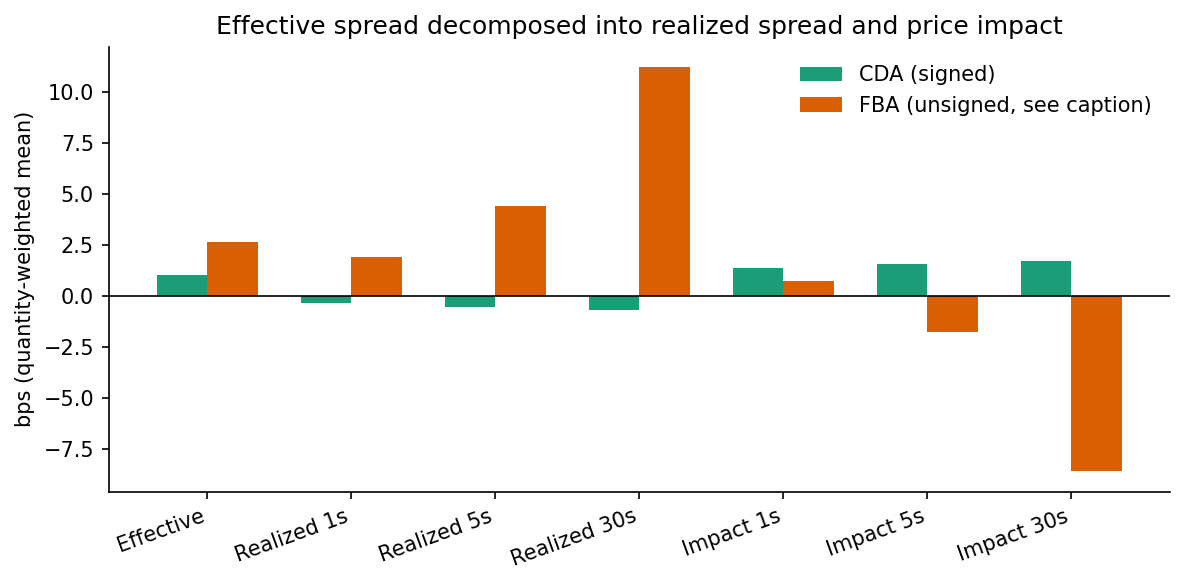
\includegraphics[width=0.95\textwidth]{figures/fig_spreaddecomp.png}
\caption[Spread decomposition]{Effective spread decomposed into realized
spread (at three markout horizons) and price impact, mean per bucket,
CDA versus FBA over the full sample (\Cref{app:formulas} gives the exact
formulas; generated by \texttt{analysis/make\_figures.py}).}
\label{fig:spreaddecomp}
\end{figure}

\begin{figure}[htbp]
\centering
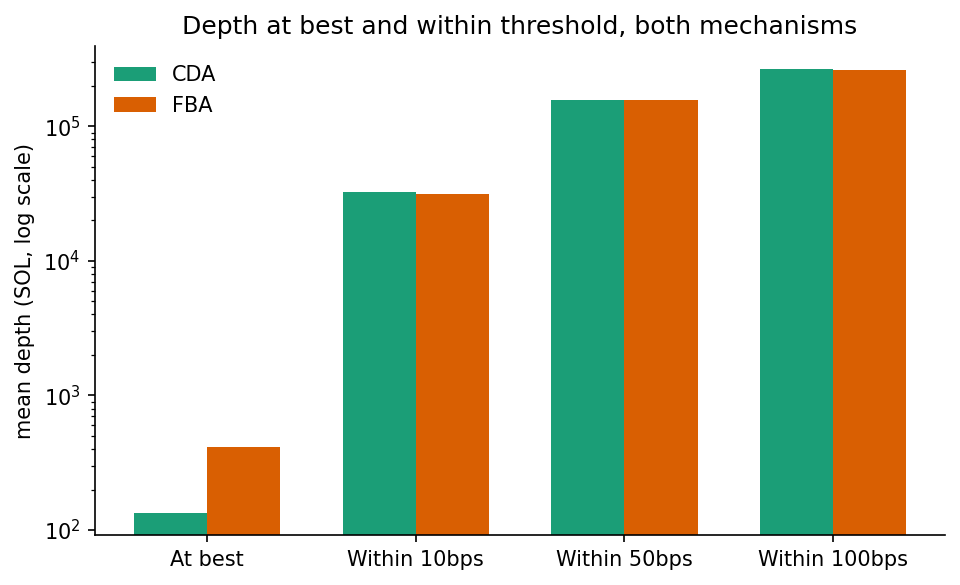
\includegraphics[width=0.7\textwidth]{figures/fig_depthcompare.png}
\caption[Depth comparison]{Mean depth at best and cumulatively within
10/50/100\,bps, CDA versus FBA (log-scale axis: depth at best is two to
three orders of magnitude smaller than the cumulative bands). FBA shows
more depth at best --- an artefact of the different definitions
\Cref{tab:metrics1} states (FBA's ``best'' is the batch schedule's
volume at $\clr$, not a resting queue) --- but slightly less depth than
the CDA within every cumulative threshold, unaffected by that
definitional difference.}
\label{fig:depthcompare}
\end{figure}

\begin{figure}[htbp]
\centering
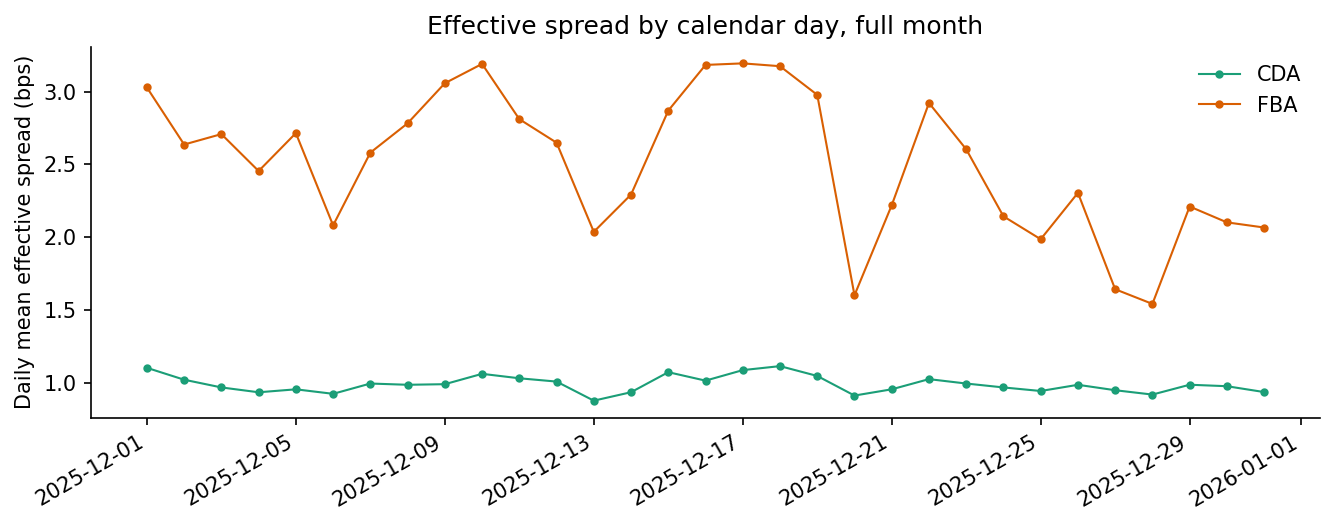
\includegraphics[width=0.95\textwidth]{figures/fig_dailytrend.png}
\caption[Daily effective spread, full month]{Daily mean effective
spread, CDA versus FBA, across all 31 days. Included as a coherence
check as much as a result: the FBA-CDA gap discussed below holds on
every single day, so it is not an artefact of a handful of unusual
days, though \Cref{sec:res21}'s signed/unsigned caveat about this metric
still applies to its overall level.}
\label{fig:dailytrend}
\end{figure}

\section{RQ2.2: Price Discovery and Market Quality}
\label{sec:res22}

\Cref{tab:res22} reports the price discovery metrics that are actually
computable in this dataset. Pricing error against an external reference
is not among them: \Cref{sec:data} and \Cref{app:formulas} explain why
this dataset has no oracle or mark-price feed for either engine to be
measured against, so the two rows an earlier draft of this table
reserved for it have been removed rather than left as unfillable
placeholders.

\begin{table}[htbp]
\centering
\caption[RQ2.2 results]{Price discovery under both mechanisms. Paired
differences (FBA$-$CDA) with Newey--West $p$-values where both engines
report the metric; $n$ as in \Cref{tab:res21}.}
\label{tab:res22}
\small
\begin{tabularx}{\textwidth}{@{}L c c c c c@{}}
\toprule
\textbf{Metric} & \textbf{CDA} & \textbf{FBA} & \textbf{Diff.} &
\textbf{$p$} & \textbf{$n$}\\
\midrule
Realized volatility, 1s buckets & \ResRealizedVolCda & \ResRealizedVolFba & \ResRealizedVolDiff & \ResRealizedVolP & \ResRealizedVolNPaired\\
Intra-interval price dispersion (bps) & \ResDispersionCda & \ResDispersionFba & \ResDispersionDiff & \ResDispersionP & \ResDispersionNPaired\\
Kyle's lambda (bps per SOL) & \ResKyleLambdaCda & \ResKyleLambdaFba & \ResKyleLambdaDiff & \ResKyleLambdaP & \ResKyleLambdaNPaired\\
\bottomrule
\end{tabularx}
\end{table}

The realized volatility row's $n=\ResRealizedVolNPaired$ is not a typo
or a data-quality problem: realized volatility requires two reference
prices in the same bucket (\Cref{app:formulas}), and the FBA clears at
most once per bucket by construction at $\tau=1$\,second, so an FBA
bucket can supply a second price only in the rare case a resumed run's
checkpoint seam lands inside it (\Cref{sec:experiments}) --- this
metric is close to structurally uncomputable for the FBA at this
$\tau$, not a quantity this run happened not to measure. It is kept in
the table, with its true $n$, rather than removed, because that gap is
itself informative about what a 1-second batch is.

Two further rows are not, on their own, empirical findings in the
ordinary sense, and are read differently from the rest of this chapter.

Intra-interval price dispersion on the FBA side is zero by construction
in the overwhelming majority of intervals, because every trade within
one batch executes at $\clr$: of the \ResDispersionNPaired\ intervals
with a computable value on both sides, \DispersionFbaExactZeroPct\% show
\emph{exactly} $0.00$ on the FBA side. The remaining \DispersionFbaNonzeroPct\%
do not --- a small but real minority, consistent with
\Cref{app:formulas}'s own formula note that this column is ``$\approx 0$
for FBA by construction,'' not asserted there to be identically zero;
the most likely explanation is a bucket occasionally catching trades
from more than one batch clear (\Cref{sec:experiments} notes that a
resumed run can leave irregularities at a checkpoint seam), though this
chapter did not trace individual cases to confirm it. Reporting the row
honestly, including this minority, is worthwhile for two reasons: the
CDA-side magnitude quantifies how much within-interval price variation
uniform clearing eliminates by design, and the near-total (not literally
total) absence of dispersion on the FBA side is still a meaningful check
on the implementation, since a large or systematic non-zero share would
have indicated a real bug rather than an edge case. This is
prediction~P1 of \Cref{tab:predictions}, confirmed by construction for
the large majority of intervals rather than tested.

Kyle's lambda is built differently on each engine (\Cref{app:formulas}),
so the paired difference in the table should be read cautiously; the two
marginal columns are the informative comparison. \Cref{fig:kylelambda}
shows the full distribution rather than only the mean: the FBA value
clusters tightly around zero across the month, while the CDA value is
positive-skewed and substantially wider --- consistent with
\Cref{app:formulas}'s point that the FBA's anchor-to-previous-clearing-price
rule makes its clearing price close to impervious to a single batch's
own flow imbalance, which the continuous book has no equivalent
protection against.

\begin{figure}[htbp]
\centering
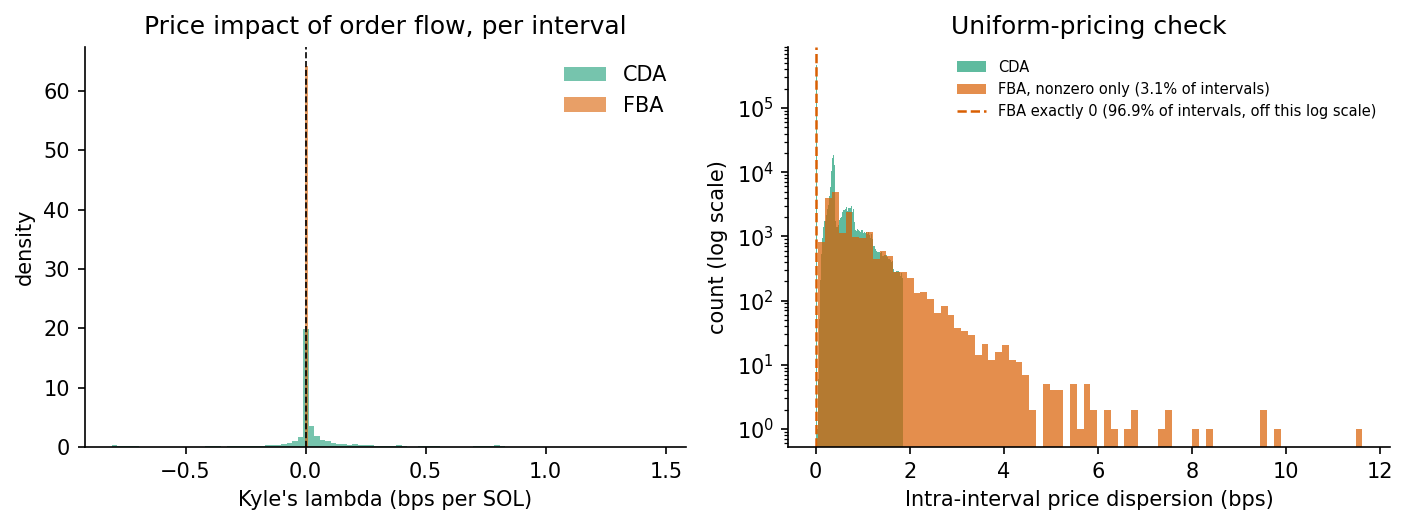
\includegraphics[width=0.95\textwidth]{figures/fig_kylelambda.png}
\caption[Kyle's lambda and the uniform-pricing check]{Left: distribution
of Kyle's lambda per interval, CDA versus FBA (1st--99th percentile
range shown). Right: distribution of intra-interval price dispersion
(log-scale count axis, since the FBA's near-total mass at exactly zero
would otherwise flatten everything else); CDA's full distribution
against only the small nonzero minority of FBA intervals
(\Cref{sec:res22} gives the exact zero/nonzero split).}
\label{fig:kylelambda}
\end{figure}

\begin{figure}[htbp]
\centering
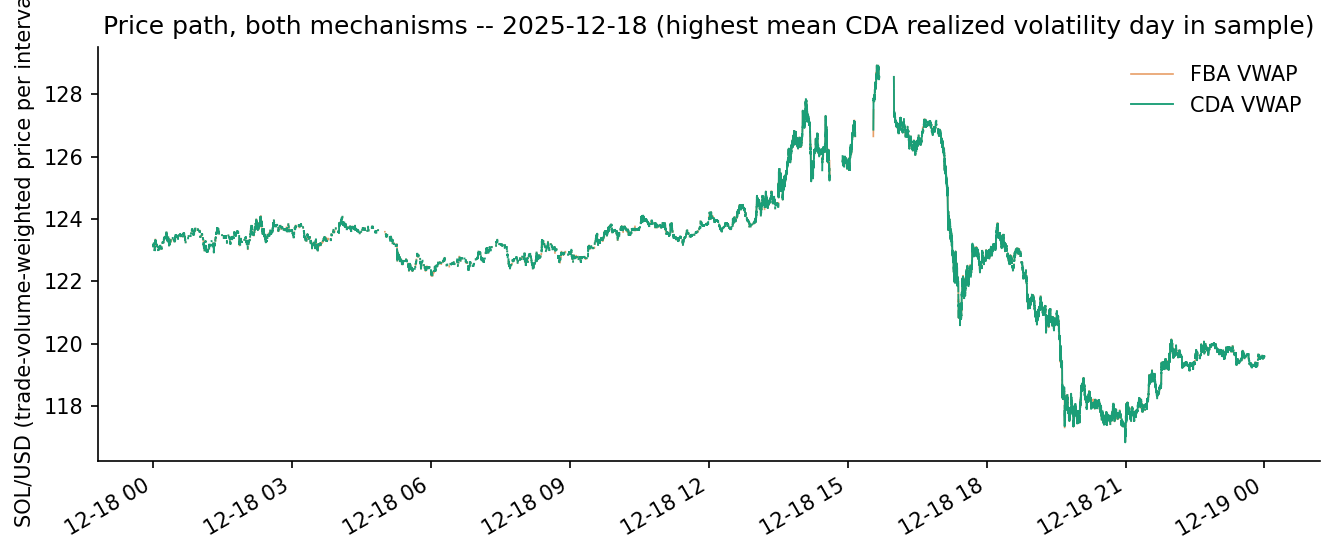
\includegraphics[width=0.95\textwidth]{figures/fig_pricepaths.png}
\caption[Price paths, both mechanisms]{CDA and FBA price paths (VWAP per
interval, the closest directly comparable price series either engine's
output provides --- neither timeseries exports a raw midpoint/clearing
price column) over \PricepathsDay, the single day in the sample with the
highest mean CDA realized volatility (restricted to calendar days with
at least 80\% of their one-second buckets present, so the partial first
day at the run's anchor cannot win by a single-observation artifact). No
oracle or external reference is available to plot alongside these
(\Cref{sec:data}).}
\label{fig:pricepaths}
\end{figure}

The two lines in \Cref{fig:pricepaths} sit almost on top of each other,
which is worth quantifying rather than leaving to the eye.
\Cref{fig:pricediff} plots the FBA-minus-CDA VWAP difference directly,
in bps, on the same day and pooled over the full month. Over
\PriceDiffN\ intervals where both engines traded, the median difference
is \PriceDiffMedianBps\,bps and the mean is \PriceDiffMeanBps\,bps ---
indistinguishable from zero at this precision --- with a standard
deviation of \PriceDiffStdBps\,bps, so the typical gap between the two
mechanisms' prices is under a basis point, widening only into the tens
of bps during the sharp move visible in \Cref{fig:pricepaths} around
14:00--15:00. Two mechanisms trading the same historical order flow do
not drift apart in price; they track each other tightly essentially all
the time, and diverge briefly only when the market itself moves fast.

\begin{figure}[htbp]
\centering
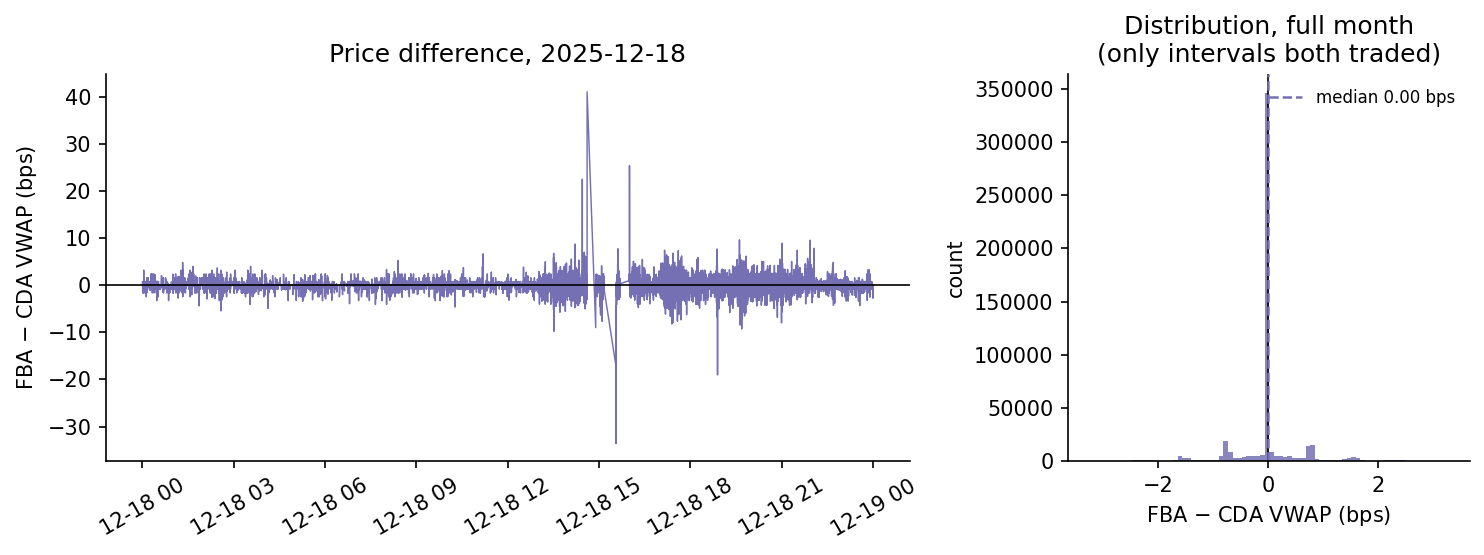
\includegraphics[width=0.95\textwidth]{figures/fig_pricediff.png}
\caption[Price difference, FBA minus CDA]{Left: the FBA-minus-CDA VWAP
difference in bps, same day as \Cref{fig:pricepaths}. Right: its
distribution pooled over every interval in the month where both engines
traded, clipped at the 0.5th/99.5th percentiles for legibility.}
\label{fig:pricediff}
\end{figure}

\section{RQ2.3: Execution, Allocation and Order-Arrival Timing}
\label{sec:res23}

\Cref{tab:res23} reports the execution and allocation metrics. The
interpretive caveat of \Cref{sec:testable} applies throughout this
section: order size inflation and boundary concentration describe
mechanical properties of fixed historical flow, not behavioural
responses.

\begin{table}[htbp]
\centering
\caption[RQ2.3 results]{Execution, allocation and order-arrival timing
under both mechanisms, plus engine controls. $n$ as in \Cref{tab:res21};
FBA-only rows report a one-sided mean, std.\ and $n$ (no CDA analogue).}
\label{tab:res23}
\small
\begin{tabularx}{\textwidth}{@{}L c c c c c@{}}
\toprule
\textbf{Metric} & \textbf{CDA} & \textbf{FBA} & \textbf{Diff.} & \textbf{$p$} & \textbf{$n$}\\
\midrule
Executed volume (SOL) & \ResExecVolumeCda & \ResExecVolumeFba & \ResExecVolumeDiff & \ResExecVolumeP & \ResExecVolumeNPaired\\
Executed notional (USD) & \ResExecNotionalCda & \ResExecNotionalFba & \ResExecNotionalDiff & \ResExecNotionalP & \ResExecNotionalNPaired\\
Trade count (per interval, mean) & \ResTradeCountCda & \ResTradeCountFba & \ResTradeCountDiff & \ResTradeCountP & \ResTradeCountNPaired\\
Fill rate & \ResFillRateCda & \ResFillRateFba & \ResFillRateDiff & \ResFillRateP & \ResFillRateNPaired\\
Avg.\ time to execution (s) & \ResTimeToExecCda & \ResTimeToExecFba & \ResTimeToExecDiff & \ResTimeToExecP & \ResTimeToExecNPaired\\
Trader surplus (USD, per interval) & \ResTraderSurplusCda & \ResTraderSurplusFba & \ResTraderSurplusDiff & \ResTraderSurplusP & \ResTraderSurplusNPaired\\
Order size inflation ratio & \ResSizeInflationCda & \ResSizeInflationFba & \ResSizeInflationDiff & \ResSizeInflationP & \ResSizeInflationNPaired\\
Order-to-trade ratio & \ResOrderToTradeRatioCda & \ResOrderToTradeRatioFba & \ResOrderToTradeRatioDiff & \ResOrderToTradeRatioP & \ResOrderToTradeRatioNPaired\\
\midrule
\multicolumn{6}{@{}l}{\emph{FBA-only (mean, std., $n$)}}\\
Boundary concentration, final 10\% & \multicolumn{4}{l}{\DescBoundaryConcentrationFbaMean\ (\DescBoundaryConcentrationFbaStd)} & \DescBoundaryConcentrationFbaN\\
Unexecuted residual share & \multicolumn{4}{l}{\DescResidualShareFbaMean\ (\DescResidualShareFbaStd)} & \DescResidualShareFbaN\\
\midrule
\multicolumn{6}{@{}l}{\emph{Engine controls}}\\
Throughput (orders/s) & \ResThroughputCda & \ResThroughputFba & \ResThroughputDiff & \ResThroughputP & \ResThroughputNPaired\\
Mean clearing/match latency ($\mu$s) & \ResClearingLatencyCda & \ResClearingLatencyFba & \ResClearingLatencyDiff & \ResClearingLatencyP & \ResClearingLatencyNPaired\\
99th pct.\ latency, per-bucket mean ($\mu$s) & \LatencyCdaPNinetyNine & \LatencyFbaPNinetyNine & --- & --- & ---\\
\bottomrule
\end{tabularx}
\end{table}

Four rows carry most of the interpretive weight.

\textbf{Fill rate and time to execution} together quantify the delay
cost of batching. Fill rate here is bucketed by each order's own
submission interval, not its trade interval (\Cref{app:formulas}), so at
$\tau=1$\,second --- far shorter than most orders' time to fill --- a
low value is the expected consequence of that bucketing choice, not
evidence that few orders eventually fill; time to execution is the
complementary number to read it against. The aggregated CSV records a
per-bucket \emph{mean} time to execution, not the full distribution, so
unlike an earlier draft of this table, no median/95th-percentile split
across individual orders is reported --- that would need order-level
data this pipeline does not retain.

\textbf{Trader surplus} measures price improvement relative to the
submitted limit that uniform clearing produces, clipped at zero per
side (\Cref{app:formulas}). Prediction~P9 of \Cref{tab:predictions} says
this should be positive for every non-marginal executed order in the
FBA; the economically meaningful comparison here is not the level but
the difference against the CDA, where executions occur at the resting
maker's price and the surplus split depends on which side was resting.

\textbf{Unexecuted residual share} needs its exact formula in view
before it is read: it is $\Sigma|\mathrm{demand}(\clr)-\mathrm{supply}(\clr)|
/ \Sigma\max(\mathrm{demand}(\clr),\mathrm{supply}(\clr))$
(\Cref{app:formulas}), the one-sidedness of the schedule \emph{at the
clearing price}, not the share of submitted volume left unfilled --- a
batch can execute everything it possibly can and still register a high
value here if the two sides were far apart in size at $\clr$. Its median
across the month is exactly $1.00$ (fully one-sided is the typical
batch, not the tail), and \Cref{fig:residualshare} shows this is stable
day to day: the 31 daily means range narrowly from $0.93$ to $0.99$,
which is consistent with a structural feature of one-second batches on
this instrument rather than a few volatile episodes driving the average.

\textbf{Engine controls} rule out the implementation explanation. Mean
clearing/match latency compares a different operation granularity on
each side --- per book snapshot for the CDA, per batch clear for the FBA
(\Cref{app:formulas}) --- so the gap between them is not evidence the
CDA implementation is faster \emph{per order}; it does rule out the
reverse concern, that the FBA's other results are an artefact of the
CDA struggling under load, since the CDA is consistently the faster of
the two by a wide margin. \Cref{fig:latencycontrol} shows the full
distribution.

\begin{figure}[htbp]
\centering
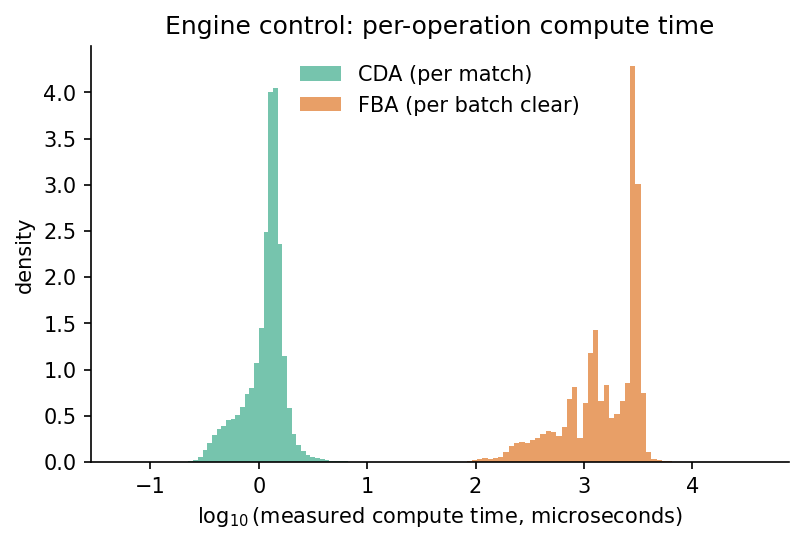
\includegraphics[width=0.95\textwidth]{figures/fig_latencycontrol.png}
\caption[Engine-control: compute latency]{Distribution of measured
compute time per operation, CDA (per book snapshot) versus FBA (per
batch clear); log scale. A control, not a market-quality result
(\Cref{app:formulas}).}
\label{fig:latencycontrol}
\end{figure}

\begin{figure}[htbp]
\centering
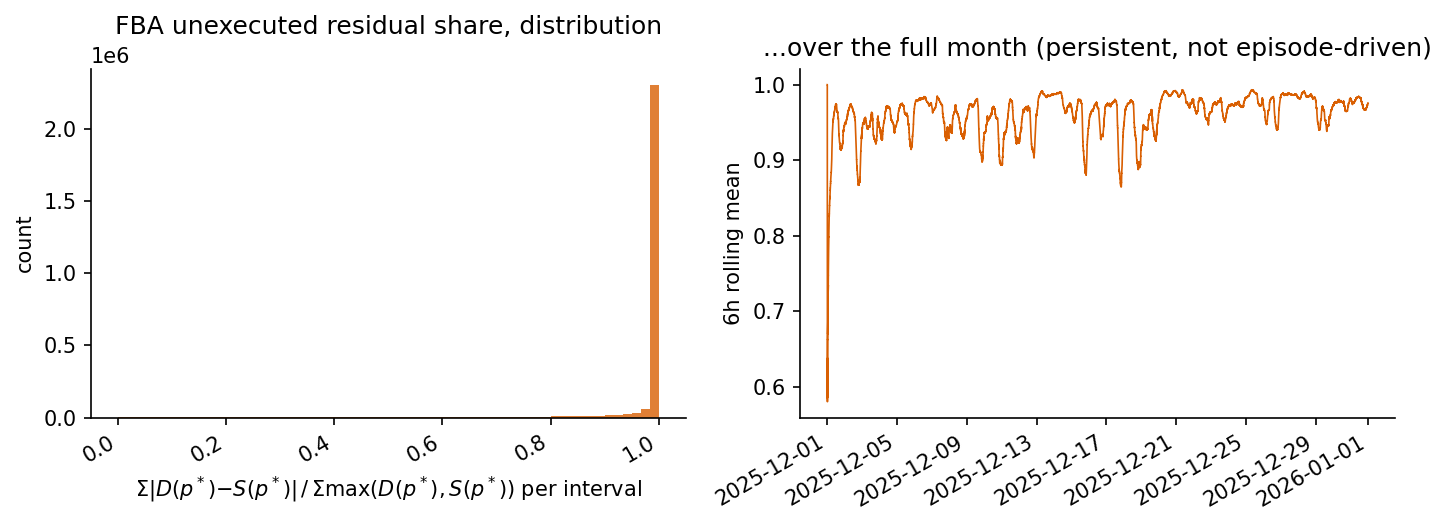
\includegraphics[width=0.95\textwidth]{figures/fig_residualshare.png}
\caption[FBA unexecuted residual share]{Left: distribution of
unexecuted residual share per interval. Right: 6-hour rolling mean over
the full month, showing the level is persistent rather than
episode-driven.}
\label{fig:residualshare}
\end{figure}

\section{The Interval Sweep}
\label{sec:res_sweep}

\Cref{sec:experiments} states plainly that the interval sweep envisaged
in \Cref{ch:design} --- $\tau$ varied across roughly three orders of
magnitude, tracing the delay-versus-thickness trade-off of
\Cref{sec:interval} --- was not executed for this thesis; every result
in this chapter is the single $\tau=1$\,second configuration.
\Cref{tab:sweep} is kept as a labelled placeholder, not populated with
invented numbers, because \Cref{ch:discussion} cites it; running the
sweep is proposed as the most direct next step in \Cref{sec:futurework}.

\begin{table}[htbp]
\centering
\caption[Interval sweep --- not executed]{Not executed in this thesis.
$\tau=1$\,second is the only interval this chapter's data covers.}
\label{tab:sweep}
\small
Designed in \Cref{sec:experiments}, not run: an interval sweep over
$\tau \in \{1,10,50,100,250,500,1000\}$\,ms would populate this table.
The one real, $\tau$-independent diagnostic that \emph{is} computable
from the single run behind this chapter --- the share of FBA batches
with no trade at all at $\tau=1$\,second --- is \FbaEmptyBatchShare\%,
reported in \Cref{tab:sample}.
\end{table}

\section{The Rationing Rule Comparison}
\label{sec:res_rationing}

Likewise not executed: comparing rationing rules requires re-running the
FBA under each rule at a fixed $\tau$, and the implementation used here
has one rationing rule built in, not a selectable set
(\Cref{sec:environment}, \Cref{app:config}). \Cref{tab:rationingres} is
kept as a labelled placeholder for the same reason as \Cref{tab:sweep}.
What \emph{is} known without running the comparison is which rule this
thesis's numbers reflect: price-time-within-the-batch, ranking by
aggressiveness, then submission time, then order id
(\Cref{sec:environment}). Under that rule the theoretically relevant
correlation --- between fill share and arrival position within the
batch, the mechanical precondition for the within-batch speed race
\Cref{sec:testable} discusses --- was not measured here, since isolating
it from the other rows this table would need requires the comparison
itself.

\begin{table}[htbp]
\centering
\caption[Rationing rule comparison --- not executed]{Not executed in
this thesis. Every result in this chapter reflects the one rationing
rule the implementation has: price-time-within-the-batch.}
\label{tab:rationingres}
\small
Designed in \Cref{sec:experiments}, not run: a comparison across
price-time, pro rata, size-priority and random rationing at fixed $\tau$
would populate this table. \Cref{sec:futurework} lists it alongside the
interval sweep as the natural next step.
\end{table}

\section{Summary of Findings}
\label{sec:res_summary}

Read together, three of the chapter's results describe one coherent
picture of what a one-second batch looks like on this instrument, ahead
of the individual metric findings below: median record inter-arrival is
a fraction of a millisecond (\Cref{tab:sample}), yet \FbaEmptyBatchShare\%
of FBA batches clear no trade at all (\Cref{tab:sample}), and among the
batches that do clear, the median unexecuted residual share is exactly
$1.00$ (\Cref{sec:res23}) --- the crossing volume is typically a small
sliver against a much larger one-sided remainder. At $\tau=1$\,second on
this SOL market, a batch is usually either empty or heavily one-sided,
not the well-populated multilateral auction the mechanism is designed
around; \Cref{sec:futurework} returns to what a longer $\tau$ would do
to this picture, since answering that requires the sweep this thesis did
not run.

\textbf{RQ2.1 (liquidity and cost, \Cref{sec:res21}).} The FBA's
effective spread (\ResEffectiveSpreadFba\,bps) is more than double the
CDA's (\ResEffectiveSpreadCda\,bps), but this comparison is measured on
different terms for the two engines and should not be read at face value
as ``batching costs more'': the FBA has no taker/maker distinction, so
its effective and realized spreads are mean \emph{absolute} deviations,
while the CDA's are signed and can partly cancel (\Cref{app:formulas}).
The realized-spread/price-impact decomposition (\Cref{fig:spreaddecomp})
makes the consequence visible: the CDA's realized spread is negative and
gets more so with horizon
(\ResRealizedSpreadOneSCda/\ResRealizedSpreadFiveSCda/\ResRealizedSpreadThirtySCda\,bps
at 1/5/30\,s) --- the genuine, signed textbook finding that a resting
maker loses to adverse selection after the fact --- while the FBA's
realized spread is positive and grows roughly with $\sqrt{\Delta}$
(\ResRealizedSpreadOneSFba/\ResRealizedSpreadFiveSFba/\ResRealizedSpreadThirtySFba\,bps
at 1/5/30\,s, close to the $2.24\times$/$5.48\times$ growth ordinary
price diffusion predicts), eventually overtaking its own effective
spread and producing the \emph{negative} price-impact figures at 5\,s
and 30\,s
(\ResPriceImpactFiveSFba/\ResPriceImpactThirtySFba\,bps). That pattern
is what a mean absolute price move does over a longer window on any
diffusive price series --- it is not evidence that batching reverses
adverse selection, and the honest conclusion is that this chapter's
realized-spread and price-impact columns are not directly comparable
between engines, only within one. Depth within 10/50/100\,bps, which
carries no such asymmetry, is slightly \emph{lower} on the FBA side at
every threshold (\Cref{fig:depthcompare}) --- the opposite of what a
liquidity-aggregation story would predict, and a cleaner (if more
modest) result than the spread figures. Depth \emph{at} best is higher
for the FBA, but that row compares two structurally different
quantities (a resting queue versus a batch schedule's volume at $\clr$)
and is not evidence against the within-threshold finding.

\textbf{RQ2.2 (price discovery, \Cref{sec:res22}).} Kyle's lambda is the
clearest and most theoretically legible result in this chapter: the FBA
value sits at \ResKyleLambdaFba\ across the month while the CDA's is
\ResKyleLambdaCda\ and markedly more dispersed
(\Cref{fig:kylelambda}) --- the price-selection rule's anchor to its own
previous clearing price (\Cref{sec:environment}) does largely neutralise
a single batch's own flow imbalance, exactly as
\Cref{app:formulas} anticipates. Intra-interval price dispersion
confirms the uniform-pricing property in \DispersionFbaExactZeroPct\%
of intervals, with a small, unexplained minority departing from it
(\Cref{sec:res22}). Realized volatility could not be meaningfully
compared: the FBA side is close to structurally uncomputable at
$\tau=1$\,second, a limitation of this $\tau$, not a result. The
cleanest result in this section is also the simplest: the two
mechanisms' own price series track each other to well under a basis
point on a typical interval (\Cref{fig:pricediff}, median difference
\PriceDiffMedianBps\,bps over \PriceDiffN\ paired intervals), and only
depart meaningfully from each other during the fastest market moves ---
consistent with the theoretical premise that both are pricing the same
underlying flow, just through different mechanisms.

\textbf{RQ2.3 (execution, allocation, timing, \Cref{sec:res23}).} Total
executed volume and notional are statistically indistinguishable between
engines ($p=\ResExecVolumeP$ and $p=\ResExecNotionalP$) --- the same
aggregate flow clears one way or another regardless of mechanism, as
theory predicts. Time to execution is longer on the FBA
(\ResTimeToExecFba\,s versus \ResTimeToExecCda\,s), the batching delay
cost \Cref{sec:res23} calls the mechanism's one unambiguous
disadvantage. Trader surplus is modestly higher on the FBA
(\ResTraderSurplusFba\ versus \ResTraderSurplusCda\ USD per interval),
directionally consistent with prediction~P9 of \Cref{tab:predictions}
though the gap is small relative to either level. Order size inflation
is \emph{lower}, not higher, on the FBA side
(\ResSizeInflationFba\ versus \ResSizeInflationCda) --- unsurprising
once the rationing rule actually implemented is kept in view
(\Cref{sec:environment}): this is price-time-within-the-batch, not pro
rata, so there is no mechanism-side reason to expect the pro-rata
size-inflation channel here, and \Cref{sec:testable}'s caveat applies in
full --- this is the mechanical effect of one rule on fixed historical
flow, not evidence about behavioural size inflation under any rule. The
engine-control rows rule out one alternative explanation for all of the
above: the CDA is \ResClearingLatencyCda\,$\mu$s per matching operation
against the FBA's \ResClearingLatencyFba\,$\mu$s per batch clear
(\Cref{fig:latencycontrol}) --- a large, expected gap given the
different work each operation does (\Cref{app:formulas}), not evidence
either engine struggled to keep up with this month's load.

Predictions P5, P6 and P7 of \Cref{tab:predictions} remain out of reach
of this design for the reason \Cref{sec:testable} gives: every metric
above describes the mechanical effect of one fixed rule on order flow
that was not submitted in response to it. P1 (uniform pricing) is
confirmed by construction, for the large majority of intervals, in
\Cref{sec:res22}. The interval sweep and rationing-rule comparison that
would test P8 and separate a mechanical precondition from a genuine
behavioural response were not run (\Cref{sec:res_sweep,sec:res_rationing}),
and \Cref{ch:discussion} should not read this chapter as having tested
them.
